\documentclass[b5paper,opensource]{./template/qyxf-book}
%注意,我修改了模板里的\solve,使其后文字首行缩进两字符

% 这里可以自定义一些命令
\newcommand{\di}[1]{\mathrm{d}#1}
\newcommand{\p}[2]{\frac{\partial #1}{\partial #2}}
\newcommand{\pp}[2]{\frac{\partial ^2 #1}{\partial #2 ^2}}
\newcommand{\dy}[2]{\frac{\di{#1}}{\di{#2}}}
\newcommand{\ddy}[2]{\frac{\mathrm{d} ^2 #1}{\mathrm{d} #2 ^2}}
\newcommand{\zbj}[4]
{
	\draw (0,0) node[below left] {$ O $};
	\draw [->] (#1,0) -- (#2,0) node[right] {$ x $};
	\draw [->] (0,#3) -- (0,#4) node[right] {$ y $};
}


\usepackage{siunitx}%输入角度
\usepackage{color}
\renewcommand{\thefootnote}{\color{red}\arabic{footnote}}%更改脚注格式
\usepackage[version=4]{mhchem}%写化学式
\newcommand{\RNum}[1]{\uppercase\expandafter{\romannumeral #1\relax}}%罗马数字
\newenvironment{mymathfrac}[2]{\left.\raise0.5ex\hbox{$#1$}\! \big\left/ \! \lower0.5ex\hbox{$#2$}\right.}%长斜分数线环境
%还需要长的\bar


\begin{document}
	
\setcounter{chapter}{10}

\chapter{热力学基础}
\section{选择题}
\exercise C

\solve 
等体加热内能增大,A错;

等温过程内能不变,$\Delta E = 0$,$Q+A>0$,$Q<0$,B错;

由$PV=nRT$,$V\uparrow$,则$T\uparrow$,则$\Delta E>0$,又$A<0$,则$Q>0$,C正确;

绝热压缩,$A>0$,$Q=0$,则$\delta E>0$,D错。

\exercise A

\solve 
由容积不变知为等体过程,则${Q_V} = \nu {C_V}({T_2} - {T_1})$,$H_2$为双原子分子,${C_V} = \frac{5}{2}R,$ \ce{NH3}为多原子分子,$C_V=3R$(本章未提及),则A正确。


\exercise B

\solve 由图中ab及cd围成面积知$\Delta {E_{ab}} = \Delta {E_{cd}}$,$A_{ab} < {A_{cd}}$,由$\Delta E = Q + A$知$Q_{ab} > {Q_{cd}}$,又${Q_{ab}}= 0$,所以${A_{cb}} < 0$,即$C < 0$,故选B。


\exercise D

\solve 等温:$\delta T=0$

等压:由$PV=nRT$,$\frac{V_2}{V_1}=\frac{T_2}{T_1}\Rightarrow \left|\delta T\right|=T_1$

绝热:由$TV^\gamma=C_2$知$(\frac{V_1}{V_2})^{\gamma-1}=\frac{T_2}{T_1}\Rightarrow \left|\delta T\right|=\left|[1-(\frac{1}{2})^{\gamma-1}]T_1\right|$

则选D。

\exercise D

\solve 绝热线与等温线只有一个交点,A错;

由$PV=nRT$,两者内能变化量相同,但做功不同,则吸热量不同,B错;

曲线下围成面积不同,C错;

由$PV=nRT$,D对。

\exercise D

\solve 等压过程,系统对外做功$A=\nu R(T_2-T_1)$,吸热$Q_P=\nu C_P(T_2-T_1)$,则$\frac{W}{Q}=\frac{A}{Q_P}=\frac{R}{C_P}=\frac{1}{1+\frac{5}{2}}=\frac{2}{7}$

故选D。

\exercise C

\solve $\eta=1-\frac{T_1}{T_2}$,易知BCC'和ADD'分别为等温线,则$\eta_1=\eta_2$;
由图,BCD下面积小于BCD',则$W_1<W_2$,故选C。

\exercise C

\solve 体积增大,则W>0;

$T_a=\frac{2p_1V_1}{nR}=T_b$,则$\Delta E=0$,故选C。

\exercise B

\solve A错,绝热斜率应该比等温线绝对值大;

B是合理的;

C、D选项,绝热线不能相交;

故选B。

\exercise D

\solve 假设可行,则$\eta=1000/1600=62.5\%$;

而由卡诺循环,$\eta=1-\frac{T_2}{T_1}=25\%$,故选D。

\section{计算题}
\exercise $\frac{1}{2}(\frac{C}{V_1^2}-\frac{C}{V_2^2})$或$\frac{1}{2}(P_1V_1-P_2V_2)$\qquad 减少\qquad 放热

\solve $W = \int_{{V_1}}^{{V_2}} {p\di{V} = } \int_{V_1}^{V_2}{\frac{C}{{{V^3}}}\di{V}=}- \frac{1}{2}(\frac{C}{{{V_2}^2}}-\frac{C}{{{V_1}^2}})=\frac{1}{2}(P_1V_1-P_2V_2)$

由$PV = nRT,P{V^3} = C$得$T=\frac{C}{nRV^2}$,V增加,T减少,则气体内能减少

$\Delta E = \nu {C_V}({T_2}-{T_1})= \frac{{{C_V}({p_2}{V_2} - {p_1}{V_1})}}{R} = \frac{C_V}{R}(\frac{C}{V_2^2}-\frac{C}{V_1^2})$

$\Delta Q = \Delta  + A = (\frac{C_V}{R} - \frac{1}{2})(\frac{C}{V_2^2} - \frac{C}{V_1^2}) < 0$

所以放热。

\exercise 不重合\qquad$\gamma$不同\qquad 不重合

\solve
$\gamma$不同,则其函数型$pV^\gamma=C$不同。

\exercise 500\qquad700

\solve 
等压过程中,$A=p\Delta V=\nu \Delta T$,单原子分子$C_{P1}=\frac{5}{2}R$

$Q_1=\nu C_{P1} \Delta T=\dfrac{5}{2}A=500\mathrm{J}$

$Q_2=\nu C_{P2} \Delta T=\dfrac{7}{2}A=700\mathrm{J}$

\exercise 温度\qquad 过程\qquad 做功\qquad 传递热量

\exercise 2/3\qquad$2S_1$

\solve
$\eta =1-\frac{T_0}{3T_0}=\frac{2}{3}$

$W=\frac{S_1}{1-\eta}-S_1=2S_1$

\exercise 1/3\qquad200J

\solve
$\eta =1-\frac{T_2}{T_1}=\frac{1}{3}$

$W=\frac{T_2}{T_1-T_2}=2\mathrm{J}$

$A=\frac{Q_2}{W}=200\mathrm{J}$

\exercise =\qquad >

\solve 两种气体对外做功即为abcda围成的面积,相等。

$\eta=\frac{W}{Q},W$相同,由$pV=nRT$知温度变化量也相同;

ab过程为等压过程,且$C_{\text{\RNum{1}}}<C_\text{\RNum{2}}$,则$Q_{\text{\RNum{1}}}<Q_{\text{\RNum{2}}}$,则有$\eta_{\text{\RNum{1}}}>\eta_{\text{\RNum{2}}}$

\exercise $\frac{1}{2}p_0V_0\qquad 9p_0V_0$

\solve W即为1\to2\to3\to1围成的面积,易得$W=\frac{1}{2}p_0V_0$

$\Delta E=\nu C_V\Delta T=\frac{3C_Vp_0V_0}{R}=\frac{15p_0V_0}{2}$

对外做功为1\to2下的面积,即$A=\frac{3p_0V_0}{2}$,则$Q=\Delta E+A=9p_0V_0$

\exercise 3R

\solve
%gxf对原解答做了改动
$A=\frac{3p_1V_1}{2}$,$\Delta T=\frac{\Delta(PV)}{\nu R}=\frac{3p_1V_1}{R}$

$\Delta E=\nu C_V\Delta T=\frac{15p_1V_1}{2}$

$Q=\Delta E+A=9p_1V_1$

\therefore$C=\frac{Q}{\Delta T}=3R$

\exercise 40J\qquad 120J

\solve 由EBCE循环系统对外做功70J,EDAE过程外界对系统做功30J,则一次循环过程系统对外做净功40J;

由于AEB为绝热过程,则$Q_{EAB}=0$,由$Q=\Delta E+A$知:

$W+\Delta E=Q_{BC}+Q_{CED}+Q_{DA}$

由于理想气体一次循环中的内能不变,则$\Delta=500$,则有$40=-30+Q_{CED}-50$,则
$Q_{CED}=120\mathrm{J}$

又因为CED为等体过程,则$A_{CED}=0,\Delta E=120\mathrm{J}$.

\section{解答题}

\exercise

\solve 由\[Q = \Delta E + A\]

知\[\eta=1-\frac{{\Delta {E_{BC}} + {A_{BC}}}}{{\Delta {E_{DA}} + A{  _{DA}}}}\]
\[{A_{BC}}=-\frac{1}{2}({p_B} + {p_C})({V_B} - {V_C})\]
\[\Delta {E_{BC}} = \nu {C_V}({T_C} - {T_B}) = \frac{{{C_V}({p_C}{V_C} - {p_B}{V_B})}}{R} = \frac{1}{{\gamma  - 1}}({p_C}{V_C} - {p_B}{V_B})\]
\[ \Rightarrow {Q_{BC}} = \frac{{\gamma  + 1}}{{2(\gamma  - 1)}}({p_C}{V_C} - {p_B}{V_B}) - \frac{1}{2}({p_C}{V_B} - {p_B}{V_C})\]
由于\[\frac{{{p_C}}}{{{V_C}}} = \frac{{{p_B}}}{{{V_B}}}\]
所以\[{p_C}{V_B} = {p_B}{V_C}\]
则\[{Q_{BC}} = \frac{{\gamma  + 1}}{{2(\gamma  - 1)}}({p_C}{V_C} - {p_B}{V_B})\]
同理\[{Q_{DA}} = \frac{{\gamma  + 1}}{{2(\gamma  - 1)}}({p_A}{V_A} - {p_D}{V_D})\]
则\[\eta  = 1 + \frac{{{Q_{BC}}}}{{{Q_{DA}}}} = 1 + \frac{{{T_C} - {T_B}}}{{{T_A} - {T_D}}}\]
在绝热过程AB中\[{T_B}{V_B}^{\gamma  - 1} = {T_A}{V_A}^{\gamma  - 1}\]
\[{p_B}^{\gamma  - 1}{T_B}^{ - \gamma } = {p_A}^{\gamma  - 1}{T_A}^{ - \gamma }\]
则有\[{T_B}^{\gamma+1}{\left(\frac{V_B}{p_B}\right)^{\gamma  - 1}} = {T_A}^{\gamma  + 1}{\left(\frac{V_A}{p_A}\right)^{\gamma  - 1}}\]
则\[\frac{{{T_B}}}{{{T_A}}} = \sqrt[{\gamma+1}]{{{{\left(\frac{V_A/p_A}{V_B/p_B}\right)}^{\gamma  - 1}}}} = \sqrt[{\gamma  + 1}]{{{{\left(\frac{V_D/p_D}{V_C/p_C}\right)}^{\gamma-1}}}} = \frac{{{T_D}}}{{{T_C}}}=k\]
则\[\eta  = 1 + \frac{T_C-T_B}{T_A-T_D} = 1 - \frac{T_B}{T_A}\]

\exercise

\solve

(1)
\begin{gather*}
A = \int_{{V_0}}^{6{V_0}} p\di{V}=7{p_0}{V_0}\\
\Delta E = \nu {C_V}({T_C} - {T_A}) = \frac{{5\nu R({T_C} - {T_A})}}{2} = \frac{5}{2}(6{p_0}{V_0} - 3{p_0}{V_0}) = \frac{{15}}{2}{p_0}{V_0}\\
Q = \Delta E + A = \frac{{29}}{2}{p_0}{V_0}
\end{gather*}
(2)
\[\di{S}=\frac{\di{Q}}{T}\footnote{该公式会在下一章介绍。}=\frac{{dE +p\di{V}}}{T}=\frac{{\nu{C_V}}}{T}\di{T}+\frac{{\nu R}}{V}\di{V}\]
则
\begin{align*}
\Delta S&= \int_{T_1}^{{T_2}}\frac{{\nu {C_V}}}{T}\di{T}+\int_{{V_1}}^{{V_2}} {\frac{{\nu R}}{V}\di{V}}\\
&=\frac{{5\nu R}}{2}\ln\frac{6{p_0}{V_0}/\nu R}{3{p_0}{V_0}/\nu R}+\nu R\ln \frac{{6{V_0}}}{{{V_0}}}\\
&= 29.29\mathrm{J/K}
\end{align*}

\exercise

\solve
(1)
\begin{figure}[!h]
	\centering
	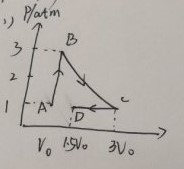
\includegraphics[width=0.35\textwidth]{Chp11_23.jpeg}
\end{figure}

(2)%gxf对原解答做了改动
\[\nu  = \frac{m}{M} = 0.1\mathrm{mol}\]
\[\frac{T_B}{T_A}=\frac{p_B}{V_B}{p_A}{V_A} = 3 \Rightarrow {T_B} = 3{T_A} = 900\mathrm{K}\]
同理,$\frac{T_D}{T_C}=0.5$,且有$T_C=T_B$,则:
\[\Delta E =\nu {C_V}({T_D}-{T_A})= 311\mathrm{J}\]
\[A =\nu R{T_B}\ln \frac{3{V_0}}{V_0}-\frac{{3P_0V_0}}{2}\]
由${p_0}{V_0} = nR{T_A}$得:
\[\frac{{3{p_0}{V_0}}}{2} = 374.13\mathrm{J}\]
则\[A = 450.65\mathrm{J}\]
\[Q = \Delta E+A = 762.42\mathrm{J}\]

\exercise

\solve 由下一章知识,\[{C_V} = \frac{i}{2}R,{C_p} = \frac{{i + 2}}{2}R\]
则
\[\gamma=\frac{{i + 2}}{i}\]
因为是绝热过程,则有
\[{T_0}{V_0}^{\gamma-1}={T_\text{\RNum{1}}}{(\frac{V_0}{2})^{\gamma-1}}= {T_\text{\RNum{2}}}{(\frac{{3{V_0}}}{2})^{\gamma-1}}\]
解得
\[{T_\text{\RNum{1}}} = {2^{\frac{2}{i}}}{T_0},{T_\text{\RNum{2}}} = {(\frac{2}{3})^{\frac{2}{i}}}{T_0}\]
则
\[A = \frac{{\nu R}}{{\gamma-1}}({(\frac{2}{3})^{\frac{2}{i}}}{T_0} - {T_0}) + \frac{{\nu R}}{{\gamma  - 1}}({2^{\frac{2}{i}}}{T_0}-{T_0}) = \frac{{i\nu R{T_0}}}{2}[{(\frac{2}{3})^{\frac{2}{i}}} + {2^{\frac{2}{i}}} - 2]\]

\chapter{气体动理论}
\section{选择题}
\exercise B

\solve 微观上,气体温度表示气体分子的运动速度,对于单个或少数分子,温度的概念失去了意义。宏观上,气体的温度表示气体分子的平均冷热程度。

\exercise B

\solve
\begin{gather*} 
{Vp=\sqrt{\frac{2kT}{u}}}\\
{u\left(\ce{O2}\right)}>u\left(\ce{H2}\right)\\
{Vp\left(\ce{O2}\right)<Vp\left(\ce{H2}\right) } \\
\frac{Vp\left(\ce{O2}\right)}{Vp\left(\ce{H2}\right)}=\sqrt{\frac{2kT}{32}} \sqrt{\frac{2kT}{2}}=\frac{1}{4}%需要长斜杠分数线
\end{gather*}
K为常量,T相同。

\exercise C

\solve 自由度为i的分子的平均动能为ikT/2。

\exercise A

\solve

$$
\begin{aligned} \sqrt {\bar{v^{2}}} &=\sqrt{\frac{3kT}{u}} \\
u\left(\ce{H2}\right)& > u\left(\ce{H2}\right) \\
\sqrt {\bar{v^{2}}\left(\ce{O2}\right)}& = \sqrt {\bar{v^{2}}\left(\ce{H2}\right) }\\
T\left(\ce{O2}\right)&>T\left(\ce{H2}\right) 
\end{aligned}
$$

\exercise B

\solve 等温过程系统内能不变。

\exercise A

\solve

\begin{gather*}
\varepsilon_{\ce{He}}=\varepsilon_{\ce{N2}}\\
n_{\ce{He}}=n_{\ce{N2}}\quad n=\frac{N}{V}\\
\bar{\varepsilon}=\frac{3}{2}kT\\
T_{\ce{He}}=T_{\ce{N2}}\\
p=\frac{2}{3}n\bar{\varepsilon}\\
p_{\ce{He}}=p_{\ce{N2}}
\end{gather*}

\exercise A

\solve

$$
\begin{aligned} 
p V & = \nu R T \\ p V & = \frac { m } { M } R T \\
p V & = \rho R T \\
\rho & = \frac { p M } { R T }
\end{aligned}
$$

由于水滴静止,则
$$
p_{\ce{H2}} =p_{\ce{O2}}
$$

又因为T相同,则

$$
\frac { p _ {\ce{H2}} } { p _ {\ce{O2}} } = \frac { \frac { p M _ {\ce{H2}} } { R T } } { \frac { p M_{\ce{O2}}}{ R T}}=\frac{1}{16}
$$

\exercise D

\solve

$$
\begin{aligned}
 \bar { z } & = \sqrt { 2 } \pi d ^ { 2 } \bar { v } n \\ \lambda & = \frac { 1 } { \sqrt { 2 } \pi d ^ { 2 } n } 
\end{aligned}
$$

$$
\because n = \frac { p } { k T }
$$不变,$ \bar { v }$不变

$$
\bar { z } = \sqrt { 2 } \pi d ^ { 2 } \bar { v } \frac { p } { k T },p
$$变为原来的两倍

$$
\begin{array} { l } 
{ \therefore z ^ { \prime } = 2 \bar { z } } \\ 
{ \because \bar { v } = \bar { \lambda } \bar { z } } \\
 { \therefore \lambda ^ { \prime } = 2 \bar { \lambda } }
\end{array}
$$

\exercise C

\solve

$$
\begin{array} { l } 
{ 2\ce{H2O} = 2\ce{H2}+\ce{O2}}\\
{ E = v\frac{i}{2}RT} 
\end{array}
$$

对于刚性分子,双原子分子气体的i=5,多原子分子气体的i=6

$$
\begin{array} { l }
 E _ { 0 } = 2 \cdot \frac { 6 } { 2 } R T \\ E _ { 0 } ^ { \prime } = 2 \cdot \frac { 5 } { 2 } R T + \frac { 5 } { 2 } R T = \frac { 15 } { 2 } R T \\ \therefore \frac { 15 } { 2 } R T \div 6 R T = 125 \% 
\end{array}
$$

\exercise B

\solve

$$
\begin{aligned} 
\sqrt { \bar { v } ^ { 2 } } & = \sqrt { \frac { 3 k T } { u } } \\ T _ { 2 } & = \frac { 3 } { 2 } T _ { 1 } \\ T _ { 2 } = \left( \frac { 3 } { 2 } \right) ^ { 2 } T _ { 1 } & = 280 \times \frac { 9 } { 4 } = 630 
\end{aligned}
$$
\section{填空题}
\exercise 
$\int _ { v _ { 2 } } ^ { v _ { 2 } } f ( v ) N d v$
\qquad
$\frac { \int _ { v _ { 1 } } ^ { v _ { 2 } } v f ( v ) d v } { \int _ { v _ { 1 } } ^ { v _ { 2 } } f ( v )\di{v}}$
\qquad
$N \cdot \frac { 1 } { 2 } m \int _{v_1}^{v_ 2} v^2f( v )\di{v}$

\solve
(1)

$$
\begin{aligned} \frac { d N } { N } & = f ( v ) d v \\ d N & = N f ( v ) d v \\ N ^ { \prime } = & \int _ { v_1 } ^ { v _ { 2 } } N f ( v ) d v \end{aligned}
$$

(2)
$$v_1 \sim v_2 \mbox{的平均速度}=\frac{\mbox{这个区间里每个分子速度之和}}{\mbox{这个区间里分子总数}}\\= \frac { \int _ { v _ { 1 } } ^ { v _ { 2 } } v d N } { \int _ { v _ { 1 } } ^ { v _ { 2 } } d N } = \frac { N \int _ { v _ { 1 } } ^ { v _ { 2 } } v f ( v ) d v } { N \int _ { v _ { 1 } } ^ { v _ { 2 } } f ( v ) d v } = \\frac { \int _ { v _ {1 } } ^ { v _ { 2 } } v f ( v ) d v } { \int _ { v _ { 1 } } ^ { v _ { 2 } } f ( v ) d v }$$

(3)
$$\mbox{总平动动能之和=每个分子平动动能之和}= \int _ { v _ { 1 } } ^ { v _ { 2 } } \frac { 1 } { 2 } m v ^ { 2 } d N \\ =  \frac { 1 } { 2 } m N \int _ { v _ { 1 } } ^ { v _ { 2 } } v ^ { 2 } f ( v ) d v 
$$


\exercise $\frac { N _ { A } } { N _ { A } + N _ { B } } f _ { A } ( v ) + \frac { N _ { B } } { N _ { A } + N _ { B } } f _ { B } ( v )$

\solve $\frac{N_A}{N_A+N_B}$指的是A在混合气体里占比,B同理。由概率论知识可知,对概率密度求加权平均即得结果。



\exercise
$
n _ { 0 } e ^ { - \frac { m g z } { k T } }
\qquad
z = - \frac { k T \ln ^ { \frac { p } { p_0 } } } { m g }
$

\solve 由玻尔兹曼分布律:

$$
\begin{aligned} n & = n _ { 0 } e ^ { - \frac { m g z } { k T } } \\ p & = p _ { 0 } e ^ { - \frac { m g z } { k T } } \\ z & = - \frac { k T \ln ^ { \frac { p } { p _ { 0 } } } } { m g } \end{aligned}
$$

\exercise 升高\qquad 升高

\solve (1)温度应上升。因为高速运动的氧气瓶中的分子是在杂乱无章运动的基础上附加上x方向定向运动速度。氧气瓶静止下来后,气体分子与氧气瓶发生碰撞,高速的x方向定向运动动能通过分子之间的频繁碰撞逐步平均分配到y、z方向的热运动动能上去,所以温度上升。

(2)$pV=\nu RT$,$T$增大,$V,\nu,R$都不变,所以$p$增大。

\exercise $\frac{3kT}{2}$\qquad 温度是大量分子热运动的集体表现,对单个或少数分子来说,温度的概念就失去了意义。

\exercise $7.82 \times 10 ^ { 7 } s ^ { - 1 } \qquad5 \times 10 ^ { - 5 } \mathrm { cm }$

\solve
由$\bar { \lambda } = \frac { k T } { \sqrt { 2 } \pi d^2p }$,$\bar { \lambda } $和$\bar { v } $成反比.

$p _0= 1 \times 10 ^ { 5 }\mathrm{Pa}$

$p _1= 1 \times 10 ^ { 4 }\mathrm{Pa}$

${ \therefore\ \overline{\lambda^{\prime} } = 10 \bar { \lambda } = 5 \times 10 ^ { - 5 }\mathrm{ cm }}$

${ z ^{\prime } = \frac { 1 } { 10 } \bar { z } = 7.82 \times 10 ^ { 7 }\mathrm{s^{-1}}}$

\exercise 1:4:16\qquad 1:2:4

\solve

$$
\begin{array}{*{20}{c}}
 \sqrt { \bar { v } ^ { 2 } } = 1.73 \sqrt { \frac { R T } { M } } \\ \because \sqrt { \bar { v } _ { A } ^ { 2 } } : \sqrt { \bar { v } _ { B } ^ { 2 } }  : \sqrt { \bar { v } _ { C } ^ { 2 } } = 1 : 2 : 4 \\ \therefore T _ { A } : T _ { B } : T _ { C } = 1 : 2 ^ { 2 } : 4 ^ { 2 } = 1 : 4 : 16 \\ n = \frac { N } { V } = \frac { \nu N _ { A } } { V } \\ \therefore n \propto \frac { \nu } { V }\\ \therefore \frac { \nu _ { 1 } } { V _ { 1 } } : \frac { \nu _ { 2 } } { V _ { 2 } } : \frac { \nu _ { 3 } } { V _ { 3 } }  = n _ { 1 } : n _ { 2 } : n _ { 3 } = 4 : 2 : 1 \\ p V  = \nu R T \\ p = \frac { \nu R T } { V }  = \frac { \nu } { V } \cdot T \cdot R \\ \therefore p  \propto \frac { \nu } { V } T \\ \therefore p _ { 1 } : p _ { 2 } : p _ { 3 } = 4 \times 1 : 2 \times 4 : 1 \times 16 = 1 : 2 : 4  
\end{array}
$$

\exercise 6

\solve (1)刚性多原子分子(甲烷)共有6个自由度。

(2)由于分子热运动的无规则性,任何一种运动都不比其他运动占有特别的优越性,所以机会相等,所以分子绕其质心转动对$i$的贡献为3.

\exercise $\geqslant 0 $\qquad 不变 \qquad 增

\solve
(1)孤立系统的熵永远也不会减少。

(2)可逆过程熵不变。

(3)由于ΔS$\geqslant 0$,不可逆过程熵增。


\exercise 0 \qquad 增

\solve(1)气体自由膨胀,对外界不做功(A=0)。绝热过程Q=0,ΔE=-A=0。故内能增量为0。

(2)孤立系统的熵永远也不会减少。


\section{计算题}
\exercise

\solve
(1)
\begin{figure}[!ht]
	\centering
	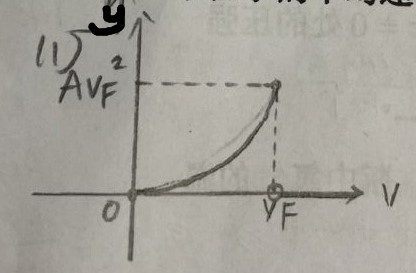
\includegraphics[width=0.35\textwidth]{./pics/Chp12_21.jpg}
\end{figure}

(2)
\begin{align*}
\int _ { 0 } ^ {+\infty}f(v)\di{v}
&=\int _ { 0 } ^ {v_F}Av^2\di{v}\\
&=\left. \dfrac { 1 } { 3 } A v ^ { 3 } \right| _ { 0 } ^ { v _ { F } }\\
&=\dfrac { 1 } { 3 } A v_F^3= 1 \\ 
A&=\dfrac{3}{ v_F^3 }
\end{align*}

(3)
速率分布曲线上与速率分布函数极大值所对应的速率称为最概然速率。

\therefore $v_P=v_F$

(4)
\begin{gather*}
{ \bar { v } = \int _ { 0 } ^ { v _ { F } } v f ( v ) d v } \\
 { \bar { v } = \int _ { 0 } ^ { v _ { F } } v \cdot \frac { 3 } { v _ { F } ^ { 3 } } v ^ { 2 } d v = \left. \frac { 3 } { 4 v _ { F } ^ { 3 } } v ^ { 4 } \right| _ { 0 } ^ { v _ { F } } = \frac { 3 } { 4 } v _ { F } } 
\end{gather*}

(5)
\begin{gather*}
 { \bar { v } = \int _ { 0 } ^ { v _ { F } } v f ( v ) d v } \\
{ \bar { v } = \int _ { 0 } ^ { v _ { F } } v \cdot \frac { 3 } { v _ { F } ^ { 3 } } v ^ { 2 } d v = \left. \frac { 3 } { 4 v _ { F } ^ { 3 } } v ^ { 4 } \right| _ { 0 } ^ { v _ { F } } = \frac { 3 } { 4 } v _ { F } } \\ { \bar { v } ^ { \prime } = \int _ { \frac { v _ { F } } { 2 } } ^ { v _ { F } } \frac { 3 } { v _ { F } ^ { 3 } } v ^ { 3 } d v = \left. \frac { 3 } { 4 v _ { F } ^ { 3 } } v ^ { 4 } \right| _ { \frac { v _ { F } } { 2 } } ^ { v _ { F } } = \frac { 3 } { 4 v _ { F } ^ { 3 } } \left( v _ { F } ^ { 4 } - \frac { 1 } { 16 } v _ { F } ^ { 4 } \right) = \frac { 45 } { 64 } v _ { F } }
\end{gather*}

\exercise

\solve
(1)
\begin{gather*}
{ p = n k T } \\ 
{ n = \frac { p } { k T } = 2.415 \times 10 ^ { 25 } } \\ 
{ n ^ { \prime } = 2.415 \times 10 ^ { 16 } } \\
 { \therefore N = 2.415 \times 10 ^ { 16 } \mbox{个} } 
\end{gather*}

(2)
$$
m _ { 0 } = \frac { M } { N _ { A } } = 5.31 \times 10 ^ { - 23 } g
$$

(3)
$$
\rho = \frac { m } { V } = \frac { N m _ { 0 } } { V } = \frac { 2.415 \times 10 ^ { 16 } \times 5.31 \times 10 ^ { - 23 } } { 10 ^ { - 9 } } \times 10 ^ { - 3 } = 1.28236 \times 10 ^ { 27 } \mathrm { kg } / \mathrm { m } ^ { 3 }
$$

(4)
$$
\bar { v } = \sqrt { \frac { 8 k T } { \pi m _ { 0 } } } = \sqrt { \frac { 8 \times 1.38 \times 10 ^ { - 23 } \times 300 } { \pi \times 5.31 \times 10 ^ { - 23 } \times 10 ^ { - 3 } } } = 446 \mathrm { m } / \mathrm { s }
$$

\exercise

\solve
(1)
$$
p = p _ { 0 } e ^ { - \frac { \mu g h } { k T } } = p _ { 0 } e ^ { - \frac { M g h } { R T } } = 0.633 p _ { 0 } = 6.45 \times 10 ^ { 4 } P a
$$
(2)
每口吸入的空气v不随海拔变化而变化。

相同质量$\rightarrow v $相同。

$pV=nRT$

忽略气温随高度变化时,T为定值。

$$
\begin{array}{l}
\therefore p_{0}\cdot 17 v =0.633p_0 \cdot x v\\
{ x = 26.7 \approx 27} 
\end{array}
$$
\exercise

\solve
(1)
$$
\begin{array} { c } { \rho = \frac { m } { V } = \frac { \nu m _ { 0 } } { V } = 11.3 g / c m ^ { 3 } } \\ { p V = \nu R T } \\ { \therefore \frac { \nu } { V } = \frac { p } { R T } = \frac { 1.01 \times 10 ^ { 3 } } { 8.314 \times 300 } = 0.405 } \\ { m _ { 0 } = \rho \frac { V } { \nu } = \frac { 11.3 } { 0.405 } = 27.9012 \approx 28 } \end{array}
$$

则可能是\ce{N2},\ce{CO},\ce{CH2=CH2}

(2)
$$
\sqrt{\bar{v^{2}}}=\sqrt {\frac{3kT}{\mu}}=1.73\sqrt {\frac{RT}{M}}=1.73\times\sqrt{\frac{8.314\times 300}{28\times10^{-3}}}=516.8\mathrm{m}/\mathrm{s}
$$

(3)
\begin{align*}
\bar{\varepsilon_{\mbox{平}}}&=\frac{3}{2}kT\\
&=\frac{3}{2}\times 1.38\times 10^{-23}\times 300\\
&=6.21\times 10^{-21}\\
\bar{\varepsilon_{\mbox{转}}}&=kT\\
&=4.14\times 10^{-21}
\end{align*}

(4)单位体积总平动动能=1个分子平均平动动能*分子数密度

$$E_{\mbox{平总}}=\bar { \varepsilon } _ {\mbox{平}}n=\bar { \varepsilon } _ {\mbox{平}}\frac{p}{kT}=6.21 \times 10 ^ { - 21 } \times \frac { 1.01 \times 10 ^ { 3 } } { 1.38 \times 10 ^ { - 23 } \times 300 } = 1515 J$$

同理,$\bar { \varepsilon } _ {\mbox{转总}}=1010J$

(5)
$$
E = \nu \frac { i } { 2 } R T = 0.3 \times \frac { 5 } { 2 } \times 8.314 \times 300 = 1870.65 J
$$

\chapter{机械振动}
\section{选择题}
\exercise A

\solve
由图可知,简谐振动的周期介于2至4之间,因此角频率介于0.5$\pi$和$\pi$之间,排除C,D。又由于带入t=2,应有$x=A=2$,故仅有A选项满足要求。

\exercise B

\solve
设弹簧振子的振动方程为$x=A\cos(\omega t+\varphi_0)$,则速度方程为$v=\frac{dx}{dt}=A\omega\cos(\omega t+\varphi_0+\frac{\pi}{2})$,故振幅增大一倍,速度亦增大一倍,选B。

\exercise C

\solve
动能与振子速度的平方成正比,且在振子速度最大时,动能等于振动总能量。因此,此时动能与动能总能量的比等于$\cos^2(\omega t+\varphi_0+\frac{\pi}{2})$。又由于此时位移大小为振幅的$\frac{1}{4}$,知$\cos(\omega t+\varphi_0)=\frac{1}{4}$,故$\cos^2(\omega t+\varphi_0+\frac{\pi}{2})=1-\cos^2(\omega t+\varphi_0)=1-\left(\frac{1}{4}\right)^2=\frac{15}{16}$,选C。

\exercise C

\solve
由图可知,$v|_{t=0}=\frac{1}{2}v_{max}$,又由于图像为余弦函数右移后图像,知速度初相位为$-\frac{\pi}{3}$。若设位移初相位为$\varphi_0$,则速度初相位为$\varphi_0+\frac{\pi}{2}=-\frac{\pi}{3}$,因此$\varphi_0=-5\frac{\pi}{6}$,选D。

\exercise A

\solve
机械振动的角速度$\omega=\sqrt{\frac{a_{max}}{x_{max}}}=\sqrt{\frac{a_m}{A}}$,因此周期$T=\frac{2\pi}{\omega}=2\pi\sqrt{A/a_m}$,A选项正确,B选项错误。\par
通过平衡位置的总能量等于动能$E=\frac{1}{2}mv{_{max}}^2=\frac{1}{2}ma{_m}A$,故CD错误,选A。

\exercise A

\solve
由于起点时刻位移为$\frac{1}{2}A$,A、B选项符合要求。又由于起始时刻向x轴负方向运动,仅有A选项满足要求。

\exercise E

\solve
动能方程只能表示速度的大小,而不能表示初始状态下速度方向,因此最后一定有两个相差$\pi$的可能初始相位,因此选E。

\exercise A

\solve
弹簧振子的劲度系数与长度反比,因此每根短弹簧的劲度系数为3k。并联以后,物体受力为三根弹簧受力之和,因此相当于一根劲度系数为9k的弹簧。因此弹簧振子的周期$T=2\pi\sqrt{\frac{m}{k'}}=\frac{2\pi}{3}\sqrt{\frac{m}{k}}$,选A。

\exercise B

\solve 
由题可知,第二个质点的加速度到达正向最大(对应位移负向最大)时,第一个质点在平衡位置向正向移动。因此第二个点比第一个落后1/4个周期,也即$\pi/2$个相位。因此选B。

\exercise B

\solve
拍频等于两个音叉固有频率的差的绝对值,因此A、B选项满足要求。又由于周期$T=2\pi\sqrt{\frac{k}{m}}$,因此挂上重物后,待测音叉的震动周期变长,频率减小。由于此时的拍频也减小,说明待测音叉的固有频率是高于标准音叉的,选B。

\section{填空题}
\exercise 不是

\solve 
见教材75页,同方向不同频率谐运动的合成后振幅随时间变化,不是简谐运动。

\exercise $0.5\mathrm{cm}$ \quad $x=0.5cos(\pi t+\pi)$

\solve
初始状态速度为0,因此处在位移负向最大状态,故振幅为0.5cm,初相位为$\pi$。又由于频率为0.5Hz,知角频率为$\pi$Hz,即振动方程为$x=0.5cos(\pi t+\pi)$
 
\exercise $\frac{\sqrt{7}}{2}$ \quad $\arctan{\frac{2\sqrt{3}}{3}}$

\solve
\begin{figure}[htbp]
\centering
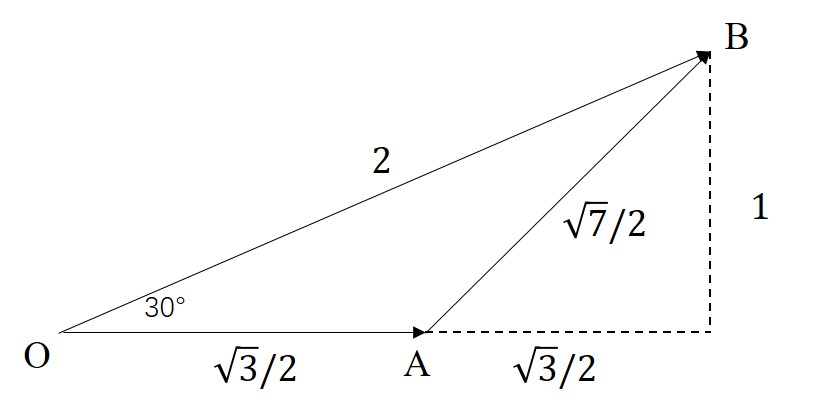
\includegraphics[height=4.7cm,width=9.5cm]{./pics/Chp13_13.jpg}
\caption{简谐运动矢量叠加图}
\end{figure}
如图绘制出简谐运动的矢量叠加图,其中OA,AB分别为第一,第二个简谐振动,OB为叠加后的简谐振动。在已知OA、AB大小方向的前提下,由几何关系即可以计算出OB的大小(即第二个简谐振动的振幅)以及两个简谐振动的相位差。

\exercise $\frac{T}{24} \quad \frac{7T}{24}$

\solve
由于速度始终比位移提前1/4个周期,而动能,势能分别与速度的平方、位移的平方成正比,因此当且仅当相位为$\pm\frac{\pi}{4}$或$\pm\frac{3\pi}{4}$ 时,动能与势能相等。因此,在半个周期内,两个动能与势能相等的时刻分别为$t_1=\frac{T}{2\pi}\left(\frac{\pi}{4}-\frac{\pi}{6}\right)=\frac{T}{24}, t_2=\frac{T}{2\pi}\left(\frac{3\pi}{4}-\frac{\pi}{6}\right)=\frac{7T}{24}$。

\exercise $0.03\cos(\frac{\pi}{2}t-\frac{\pi}{2})$

\solve
由图可知,两个简谐运动的振动方程分别为$x_1=0.06\cos(\frac{\pi}{2}t-\frac{\pi}{2})$,$x_2=-0.03\cos(\frac{\pi}{2}t-\frac{\pi}{2})$,相加后即可算出合振动的方程为$x=0.03\cos(\frac{\pi}{2}t-\frac{\pi}{2})$。

\exercise $3$

\solve
由图可知,图像为向右平移了$\frac{\pi}{3}$的余弦曲线,因此初始时刻的相位为$-\frac{\pi}{3}$,另一个x为1的点的相位与初始点关于相位为$\frac{\pi}{2}$对称,因此经过$\frac{2\pi}{3}$的角位移所需的时间为1s,由于一个周期对应$2\pi$的角位移,因此振动的周期为3s。

\exercise $\frac{3}{4}E \quad \frac{1}{4}E \quad \pm\frac{\sqrt{2}}{2}A$

\solve
弹簧振子的弹性势能与位移的平方成正比,因此当位移是振幅的一半时,弹性势能是最大弹性势能的1/4。注意到最大弹性势能与总能量$E$相等,故势能$E_p=\frac{1}{4}E$,动能$E_k=E-E_p=\frac{3}{4}E$。同理,当动能与势能相等,均为总能量一半时,位移的大小应为振幅的$\frac{\sqrt{2}}{2}$倍,即位移为$\pm\frac{\sqrt{2}}{2}A$。

\exercise $0.05\mathrm{m}\quad -\arccos{\frac{3}{5}}$

\solve
对$x$求导有$v=3A\cos(3t+\varphi+\frac{\pi}{2})$,故由题意知,$x(0)=A\cos\varphi=0.03,v(0)=3A\cos(\varphi+\frac{\pi}{2})=0.12$,联立两式即可解出$A$与$\varphi$的值。

\exercise $\sqrt{2}:\sqrt{3}$

\solve
单摆的周期$T=2\pi\sqrt{\frac{l}{g}}$,因此周期正比于绳长的平方根。由于左右两边的绳长比为2:3,周期比为$\sqrt{2}:\sqrt{3}$。

\exercise

\solve
\begin{figure}[htb]
\centering
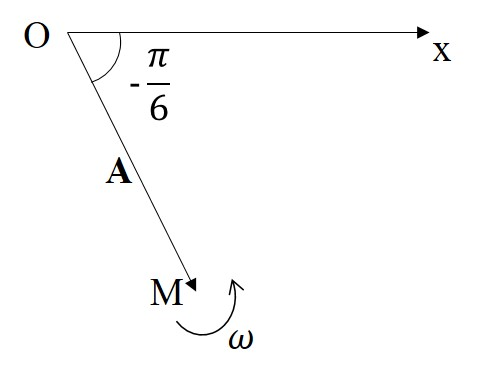
\includegraphics[height=3.7cm,width=5cm]{./pics/Chp13_20.jpg}
\caption{旋转矢量图}
\end{figure}
具体绘图方法见教材72页。

\section{计算题}
\exercise

\solve
(1)加速度$a=\frac{F}{m}=-2x$,因此角频率$\omega=\sqrt{\frac{a}{-x}}=\sqrt{2}$,故周期为$T=\frac{2\pi}{\omega}=\sqrt{2}\pi$。

(2)由于动能的最大值等于势能的最大值,有:$E_{\text{动}max}=E_{\text{势}max}=\frac{1}{2}kA^2=0.0675$J

\exercise

\solve
(1)振动的角频率$\omega=\frac{2\pi}{T}=\pi$Hz。撤去外力后,物体处于正向位移最大,负向加速度最大的状态,而撤去外力前,物体平衡。因此,撤去的外力大小等于物体振动过程中的受力最大值,即$F=ma_{max}=mA\omega^2=0.493$N

(2)弹簧的弹性系数$k=F/A=4.93$N/m,因此振动系统的总能量(与弹性势能最大值相等)为$E_{max}=\frac{1}{2}kx^2=0.0247$J。由于势能与相对平衡位置的位移的平方正比,当物体在平衡位置以下5cm,即最大位移的1/2处时,势能是最大势能(也就是总能量)的1/4,因此$E_p=\frac{1}{4}E_{max}=0.00617$J,而动能$E_ k=E_{max}-E_ p=0.0185$J

\exercise

\solve
设单摆振动方程为$x=A\cos(\omega t+\varphi_0)$,则速度方程为$v=\frac{dx}{dt}=A\omega\cos(\omega t+\varphi_0+\frac{\pi}{2})$。故由题意知,
\begin{equation*}
  \left\{
   \begin{array}{c}
   x(0)=A\cos{\varphi_0} = -5  \\
   v(0)=A\omega\cos(\varphi_0+\frac{\pi}{2}) = -10  \\
   \omega=\sqrt{\frac{g}{l}}=2.89{\rm Hz}   \\
   \end{array}
  \right.
\end{equation*}
解方程得,振幅$A=6.08$cm,初相${\varphi_0}=1.57$rad\\
另一方面,周期$T=\frac{2\pi}{\omega}=2.18$s

\exercise

\solve
以向右为正方向,设A的加速度为$a$,相对弹簧自由状态的位置为$x$。首先对A水平受力分析,A受到弹簧的力$F_1=-kx$,以及AB间绳的拉力$F_2$。为求出$F_2$,再对滑轮受力分析。滑轮转动惯量$J=\frac{mR^2}{2}$,角加速度$\beta=a/R$,右端拉力为$m_2g$,因此左端拉力$F_2=m_2g-\frac{J\beta}{R}=m_2(g-a)-0.5ma$
故A的合力$F=F1+F2=-kx+m_2(g-a)-0.5ma$,于是可以推导出a的加速度方程:
\begin{equation*}
\begin{split}
a=\frac{-kx-0.5ma+m_2(g-a)}{m_1}\\
a=\frac{-kx-0.5ma+m_2g}{m_1+m_2}\\
(1+\frac{m}{2m_1+2m_2})a=-\frac{k}{m_1+m_2}x+\frac{m_2}{m_1+m_2}g\\
a=-\frac{2k}{2m_1+2m_2+m}(x+x_0)
\end{split}
\end{equation*}
其中,$x_0=\frac{2m_2g}{2k}$。于是,角频率$\omega=\sqrt{\frac{a}{-x}}=\sqrt{\frac{2k}{2m_1+2m_2+m}}$


\end{document}
